%%Berichtvorlage für EDBV WS 2015/2016

\documentclass[deutsch]{scrartcl}
\usepackage[top=1cm,left=1cm,right=1cm,bottom=1cm]{geometry}
\usepackage[ngerman]{babel}
\usepackage[utf8]{inputenc}
\usepackage{algorithmic}
\usepackage{algorithm}
\usepackage{graphicx}
\usepackage{amsmath,amssymb}
\usepackage{subcaption}
\captionsetup{compatibility=false}
\usepackage{multirow}
\usepackage{color}

\begin{document}

\title{Verarbeitung von Grundrissen} %%Projekttitel hier eintragen

%%Namen und Matrikelnummern der Gruppenmitglieder hier eintragen
\author{Leonhard Eder (00047514), Raphael Schimmerl (00371366), \\Florian Langeder (01527111), Filip Hörtner (11808203), Mark Alam (11808580)}
\date{\vspace{-5ex}}



%%------------------------------------------------------

\maketitle

\begin{figure}[h!]
	
	\centering
	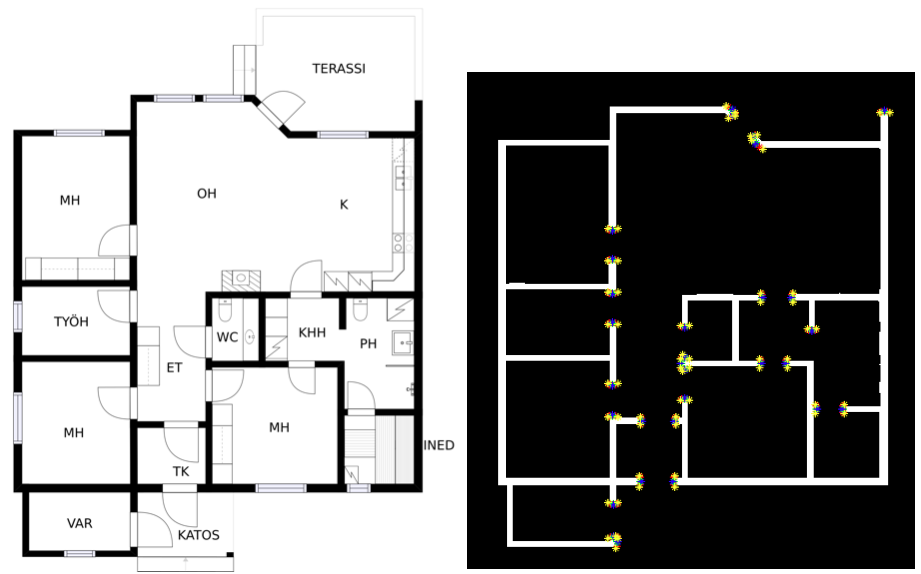
\includegraphics[width=0.8\textwidth]{mnz1.png}
	\caption{Ausgangsbild und Erkennung der Wandenden}
	\label{fig:erg}
\end{figure}

%%------------------------------------------------------

\section*{Projekt}
Ziel des Projekts ist es, bestimmte Merkmale wie Wände, Türen, Fenster, Stiegen und Räume aus einem Grundrissplan zu erkennen und diese in einem Datensatz abzuspeichern. Dieser kann zur Sortierung und Filterung von Grundrissdatensätzen verwendet werden.

\section*{Vorgangsweise}

Die Erkennungsvorgänge laufen weitgehend unabhängig voneinander ab, nur die Raumerkennung basiert auf der Abtrennung der Räume durch die Türerkennung.

\begin{enumerate}
	\item Umwandlung in ein Binärbild und Entfernung von Details
	\item Erkennung der durchschnittlichen Wandstärke
	\item Erkennung der Türen und Abtrennung der Räume
	\item Erkennung der Fenster
	\item Erkennung der Stiegen
	
\end{enumerate}

\section*{Ergebnisse}
In Abbildung \ref{fig:erg} ist zu sehen, wie die Wandenden erkannt werden. Zwei Wandenden, die sich gegenüber liegen, sind jeweils eine Tür. \\
Die Erkennung der Fenster, Türen und Räume ist in unseren Tests sehr genau, hier gibt es eine durchschnittliche Abweichung von maximal 0,5 Elementen.



\end{document}
